%!TEX root = ../template.tex
%%%%%%%%%%%%%%%%%%%%%%%%%%%%%%%%%%%%%%%%%%%%%%%%%%%%%%%%%%%%%%%%%%%
%% chapter1.tex
%% NOVA thesis document file
%%
%% Chapter with introduction
%%%%%%%%%%%%%%%%%%%%%%%%%%%%%%%%%%%%%%%%%%%%%%%%%%%%%%%%%%%%%%%%%%%

% NOTE: Cite \cite{novathesis-manual} somewhere, in your thesis/dissertation with “\verb!\cite{novathesis-manual}!”, any place you think it makes sense.  If you cite it this way, the correct entry will be added automatically to your bibliography (there no need to add it to your BibTeX file);

% epigraph configuration
% \epigraphfontsize{\small\itshape}
% \setlength\epigraphwidth{12.5cm}
% \setlength\epigraphrule{0pt}

% \epigraph{
%   This work is licensed under the \href{LaTeX project public license}{\LaTeX\ Project Public License v1.3c}.
%   To view a copy of this license, visit \url{LaTeX project public license}.
% }
\typeout{NT FILE chapter1.tex}

\chapter{Description of the Problem}
\label{cha:introduction_description}
this doesnnt even make ahahahah ahahahah ahahahah ahahahah ahahahah ahahahah ahahahah ahahahah ahahahah ahahahah ahahahah ahahahah ahahahah 
any sense

% Around twelve thousand years ago, the way of life of the average human being changed completely (until then, it simply followed primitive and sometimes unproductive ways of hunting). % citation needed
% The domestication of plants and breeding of animals started the Neolithic period, which was based on the revolution of a great base: Agriculture.
% Over the years, the agricultural exploration made possible the discovery and invention of countless phenomena and techniques, many of which are practiced and improved until the present day, since this is, precisely, a primitive area in itself.

% However, the doors of this type of exploration are far from being closed, and the machines are already able to complement and facilitate human work in the agricultural sector with much more efficiency. But there is still a great ally for such efficiency, which sometimes goes unnoticed or is even forgotten: Image Processing.


% The basic rules for writing a thesis statement are:
	% State the topic or present your argument.
	% Summarize the main idea of each of your details and/or body paragraphs.
	% Keep your statement to one to two sentences.

\section{Section 1.1}\label{sub:sub1_1}

\begin{figure}[H]
  \centering
	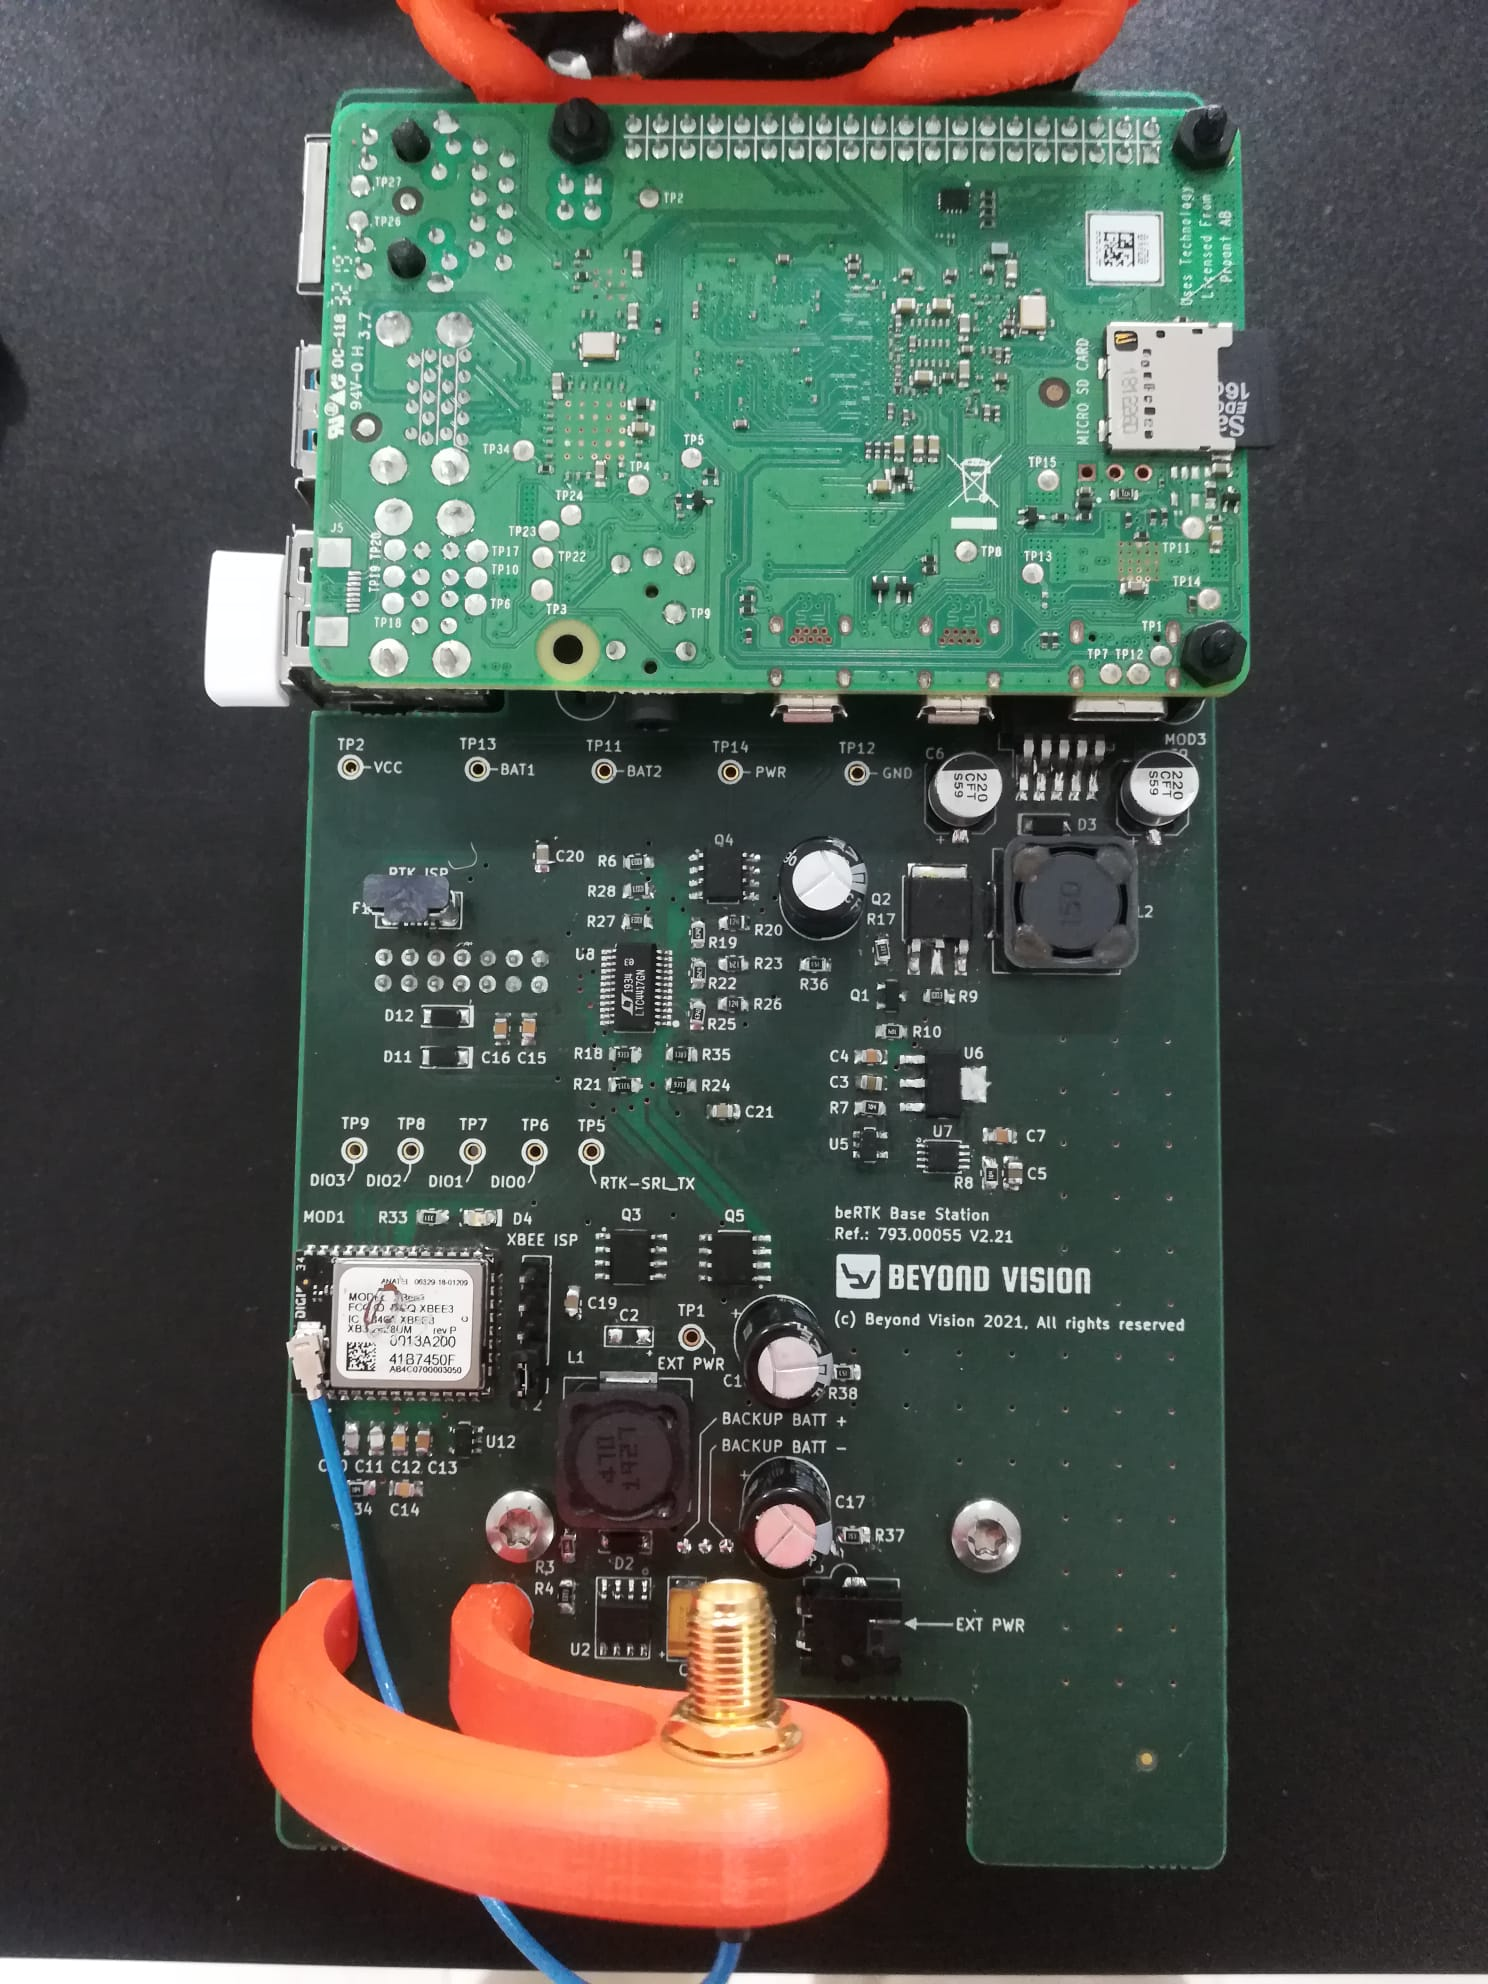
\includegraphics[width=0.5\textwidth, keepaspectratio]{Chapters/Figures/Intro/old_BS.jpeg}
	\caption{Old base station.}
	\label{fig:old_BS}
\end{figure}
This is Figure \ref{fig:old_BS}. It shows the current \gls{base_station}.

\section{Section 1.2}\label{sec:sub1_2}

\section{Section 1.3}\label{sec:sub1_3}

\section{Section 1.4}\label{sec:sub1_4}
